\documentclass[tikz,border=10pt]{standalone}
\usepackage{tikz}
\usetikzlibrary{shapes.geometric, arrows.meta, positioning, fit, backgrounds, decorations.pathreplacing, patterns}

\begin{document}
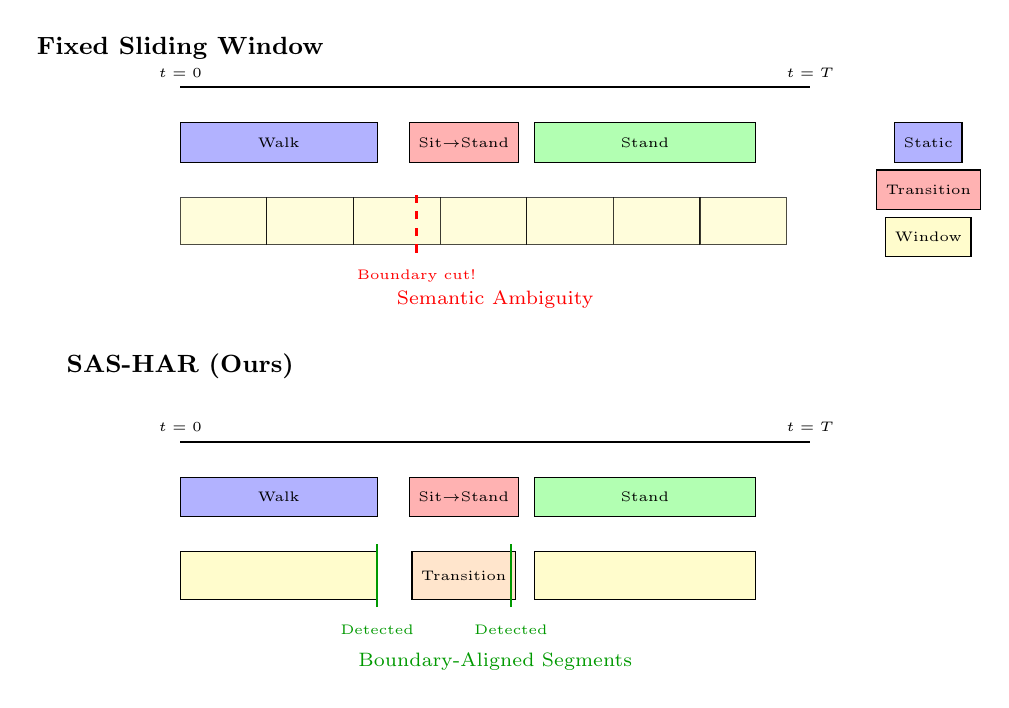
\begin{tikzpicture}[
    node distance=0.4cm,
    window/.style={rectangle, draw, minimum height=0.6cm, align=center, font=\tiny},
    activity/.style={rectangle, draw, minimum height=0.5cm, align=center, font=\tiny},
    label/.style={font=\small\bfseries}
]

% ============= FIXED SLIDING WINDOW =============
\node[label] (fswtitle) {Fixed Sliding Window};

% Timeline
\draw[thick] (0,-0.5) -- (8,-0.5);
\node[font=\tiny, above] at (0,-0.5) {$t=0$};
\node[font=\tiny, above] at (8,-0.5) {$t=T$};

% Ground truth activities
\node[activity, fill=blue!30, minimum width=2.5cm] at (1.25,-1.2) {Walk};
\node[activity, fill=red!30, minimum width=1.2cm] at (3.6,-1.2) {Sit$\to$Stand};
\node[activity, fill=green!30, minimum width=2.8cm] at (5.9,-1.2) {Stand};

% Fixed windows (misaligned)
\foreach \i in {0,1,2,3,4,5,6} {
    \node[window, fill=yellow!20, minimum width=1.1cm, opacity=0.7] at (0.55+\i*1.1,-2.2) {};
}
\draw[dashed, red, thick] (3,-2.6) -- (3,-1.8);
\node[font=\tiny, red, below] at (3,-2.7) {Boundary cut!};

\node[font=\scriptsize, text=red] at (4,-3.2) {Semantic Ambiguity};

% ============= SAS-HAR =============
\node[label, below=3.5cm of fswtitle] (sastitle) {SAS-HAR (Ours)};

% Timeline
\draw[thick] (0,-5) -- (8,-5);
\node[font=\tiny, above] at (0,-5) {$t=0$};
\node[font=\tiny, above] at (8,-5) {$t=T$};

% Ground truth activities
\node[activity, fill=blue!30, minimum width=2.5cm] at (1.25,-5.7) {Walk};
\node[activity, fill=red!30, minimum width=1.2cm] at (3.6,-5.7) {Sit$\to$Stand};
\node[activity, fill=green!30, minimum width=2.8cm] at (5.9,-5.7) {Stand};

% Adaptive windows (aligned)
\node[window, fill=yellow!20, minimum width=2.5cm] at (1.25,-6.7) {};
\node[window, fill=orange!20, minimum width=1.2cm] at (3.6,-6.7) {Transition};
\node[window, fill=yellow!20, minimum width=2.8cm] at (5.9,-6.7) {};

% Detected boundaries
\draw[thick, green!60!black] (2.5,-7.1) -- (2.5,-6.3);
\draw[thick, green!60!black] (4.2,-7.1) -- (4.2,-6.3);
\node[font=\tiny, green!60!black, below] at (2.5,-7.2) {Detected};
\node[font=\tiny, green!60!black, below] at (4.2,-7.2) {Detected};

\node[font=\scriptsize, text=green!60!black] at (4,-7.8) {Boundary-Aligned Segments};

% Legend
\node[activity, fill=blue!30, minimum width=0.8cm, font=\tiny] at (9.5,-1.2) {Static};
\node[activity, fill=red!30, minimum width=0.8cm, font=\tiny] at (9.5,-1.8) {Transition};
\node[activity, fill=yellow!20, minimum width=0.8cm, font=\tiny] at (9.5,-2.4) {Window};

\end{tikzpicture}
\end{document}
